The stagnation density inside the buffer gas cell is a function of the physical dimensions of the cell and the number flow rate into the cell. High stagnation densities allows for high densities of reactants at the ion trap center, but can push the beam into an unwanted flow regime where the beam properties are not what one wants. Experimentally, it's preferable to use volumetric flow rates when operating the apparatus, but for calculations, that needs to translate to number flow rate using the ideal gas law:

\begin{equation*}
	\dot{N} = \frac{P f}{k_B T}
\end{equation*}

where $P$ is pressure and $f$ is the volumetric flow rate, this translates to about $4\times10^{17}$particles/s$^{-1}$ for 1SCCM of gas flow. By solving for the number density in the flow out of an aperture with molecular flow, we find that the stagnation density within the cell can be shown as:

\begin{equation*}
	n_{b}=\frac{4 \dot{N}}{A_{aperture} \bar{v}}
\end{equation*}

In general, buffer gas beams operate with stagnation densities around $10^{15}-10^{17}$cm$^{-3}$. Outside of the cell, we can describe the density of the beam as a function of distance. \cite{Pauly}

\begin{equation}
	n(z)=\frac{n_0}{2}\left(1-\frac{z}{\sqrt{z^2+a^2}}\right)
\end{equation}

Where $z$ is the distance from the aperture into the vacuum side, $n_0$ is the initial number density, $a$ is the radius of the aperture. In the far-field, this goes to:

\begin{equation*}
	n(z)=\frac{n_0 a^2}{4 z^2}
\end{equation*}

But there is something that we must consider, that is that we aren't seeing the full aperture while we are at all locations, we are actually seeing an appended area due to the inclusion of apertures and skimmers in the way. So in the calculation for $n(z)$, only $n_0$ has a dependence on the aperture size of the cell, $n(z)$ itself will have a set value defined by the smallest aperture in the beam path. For us, although our cell aperture is $\approx 9$mm in diameter, we have multiple apertures and skimmers in the way, of which, a skimmer from \todo{skimmer model} with a diameter of 2mm is used.

\begin{figure}[H]
	\centering
	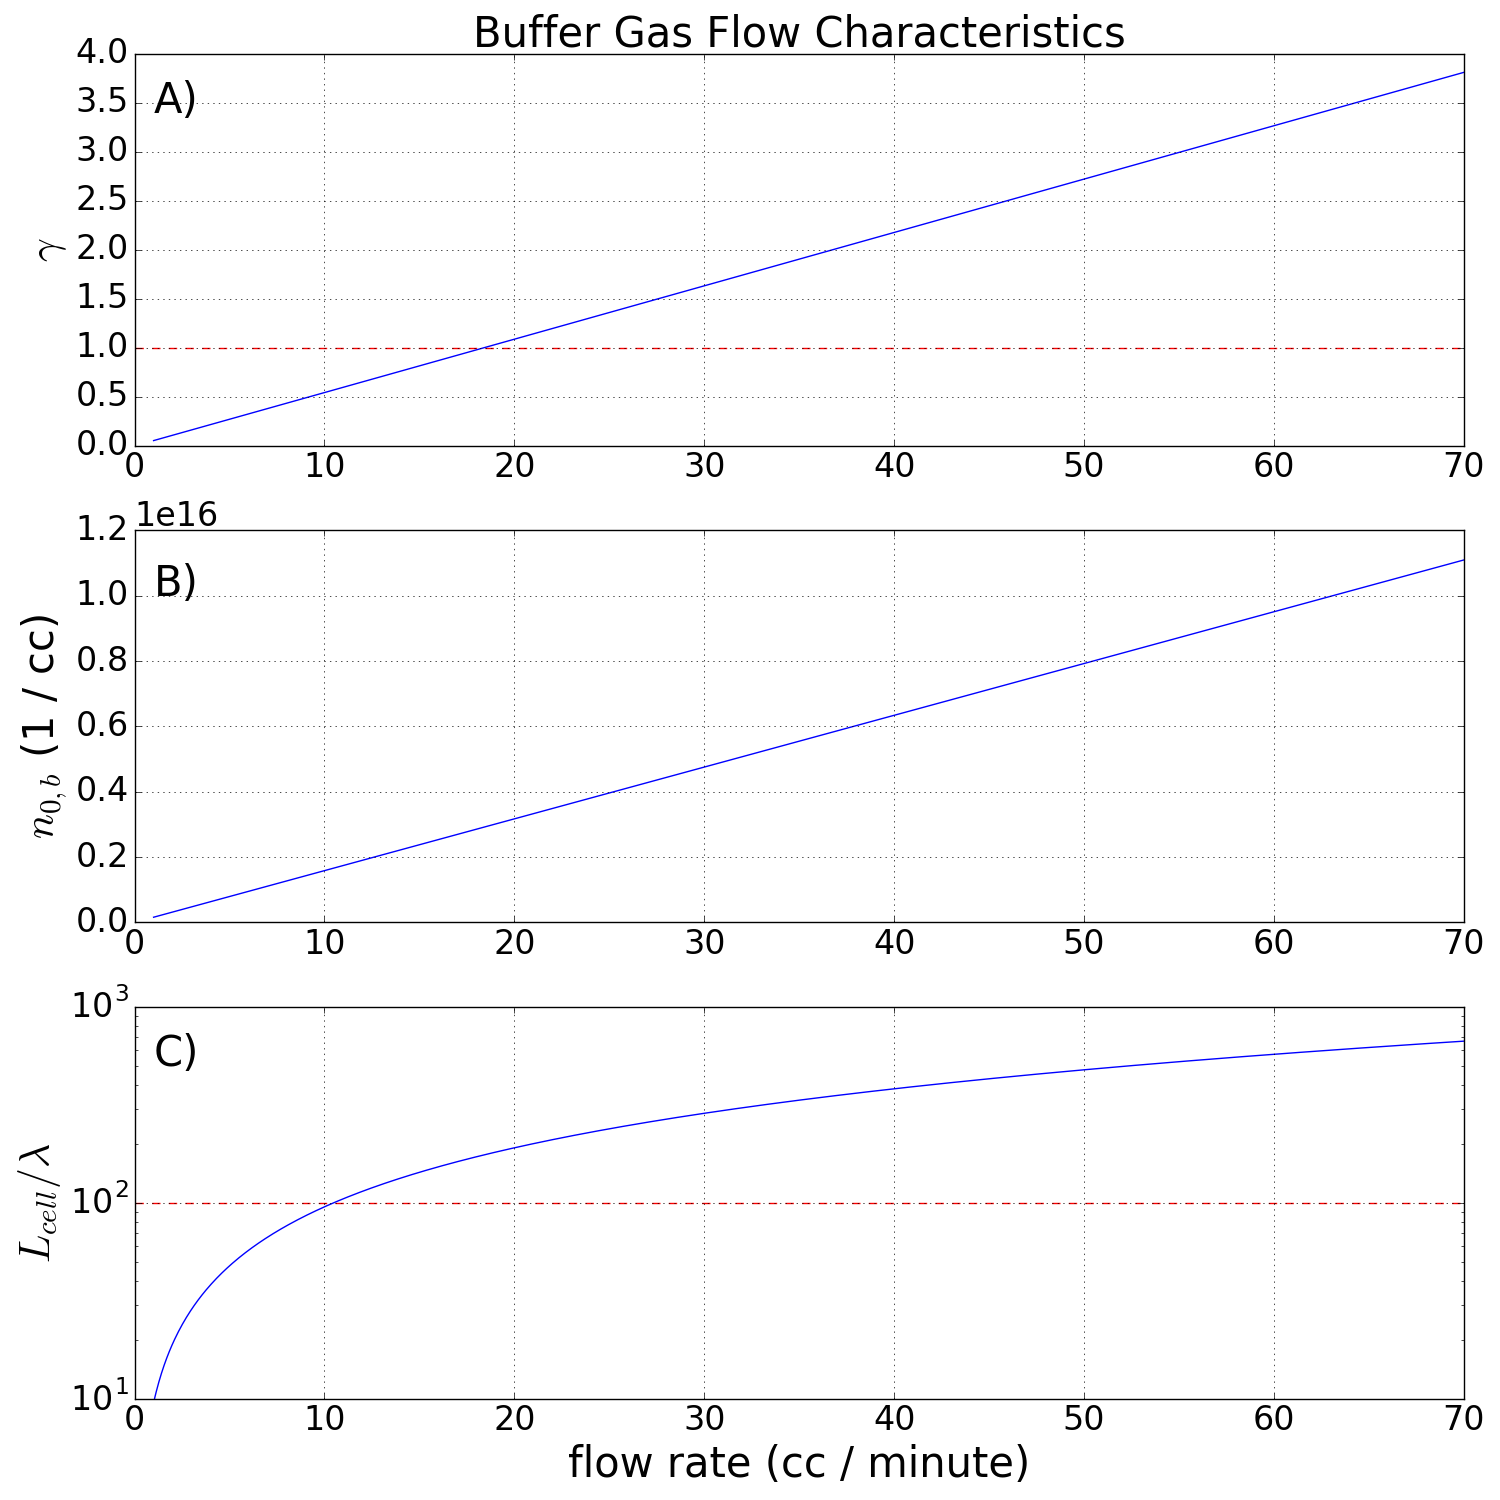
\includegraphics[width=1\textwidth]{images/CBGB_flow_characteristic.png}
	\caption{A) $\gamma$ extraction ratio, dotted red line indicates $\gamma = 1$ where hydrodynamic entrainment begins. B) Theoretical number density of buffer gas species within buffer gas cell. The density of target species introduced should stay under 1\% of the buffer gas density. C) Number of collisions a target species particle would expect before extraction out of the cell, the dotted red line indicates 100 collisions before extraction when rotational degrees of freedom are characteristically thermalized.}
	\label{f: buffer_gas_flow}
\end{figure}

Sympathetic cooling occurs through collisions between the hot target species being introduced and the cryogenic buffer gas particles. The thermalization of the target species with the buffer gas particles is derived via momentum conservation of hard sphere collisions, where $\approx 10$ and $\approx 100$ collisions are needed to relax translational and rotational states to within a factor of 2 of the buffer gas temperature. Vibrational degrees of freedom may take upwards of $10^4$ collisions to fully thermalize is the elastic collision energy is much lower than the internal vibrational level. By finding the mean free path, we can consider the characteristic length the particles travel to be thermalized with the buffer gas, this is then compared to the characteristic length of the cell to determine the effectiveness of the cooling.

\begin{equation*}
	\lambda = \frac{A_{aperture} \bar{v}}{4 f \sigma \sqrt{m_s/m_b}}
\end{equation*}

If a species is introduced into the buffer gas cell that has a lower vapor pressure than that is allowed at the current temperature, it will be lost when it comes in contact with the cell walls. The rate of this loss can be described as the  characteristic time of diffusion of a particle in the buffer gas to the physical dimensions of the cell set the diffusion time constant:

\begin{equation}
	\tau_{diff} = \frac{16}{9 \pi} \frac{A_{cell} n_{0,b} \sigma}{\bar{v}} \label{eq: tau_diff}
\end{equation}

where $\sigma$ represents the collisional cross section for the buffer gas with the target species. On the other hand, we have the characteristic pump out time given by the conductance of a cell aperture:

\begin{equation}
	\tau_{pump}=\frac{4V_{cell}}{\bar{v}A_{aperture}} \label{eq: tau_pump}
\end{equation}

By combining equations \cref{eq: tau_diff,eq: tau_pump}, we can get a dimensionless ratio, $\gamma$ that characterizes the extraction fraction out of the cell.

\begin{equation}
	\gamma = \frac{\tau_{diff}}{\tau_{pump}} = \frac{\sigma f}{L_{cell} \bar{v}} \label{eq: gamma}
\end{equation}

Notice that the $\gamma$ factor does not depend on aperture size, this is generally true, but increasing the aperture size will lower your number density within the cell, which then influences the characteristic length scale of thermalization. Larger apertures thus run the risk of not allowing your particles to fully thermalize in rotational/vibrational states. But decreasing the aperture size can make alignment as well as controlling the number density more difficult, as finer control over the flow rate is necessary for equivalent flow regimes.

We have utilized a residual gas analyzer (RGA) to determine the density of the beam in the ballistic regime upstream from the ion trap. Inserting the RGA into the beam path allows us to estimate the density of water in the beam as a function of the nominal buffer gas flow rate, as shown in figure \ref{f: rga}. Using that fit, we find good agreement with the theoretical calculations showing our flow to be near the supersonic regime, while staying in the hydrodynamic regime with a linear extraction efficiency dependence with the flow rate expressed in \ref{eq: gamma}.

\begin{figure}[H]
	\centering
	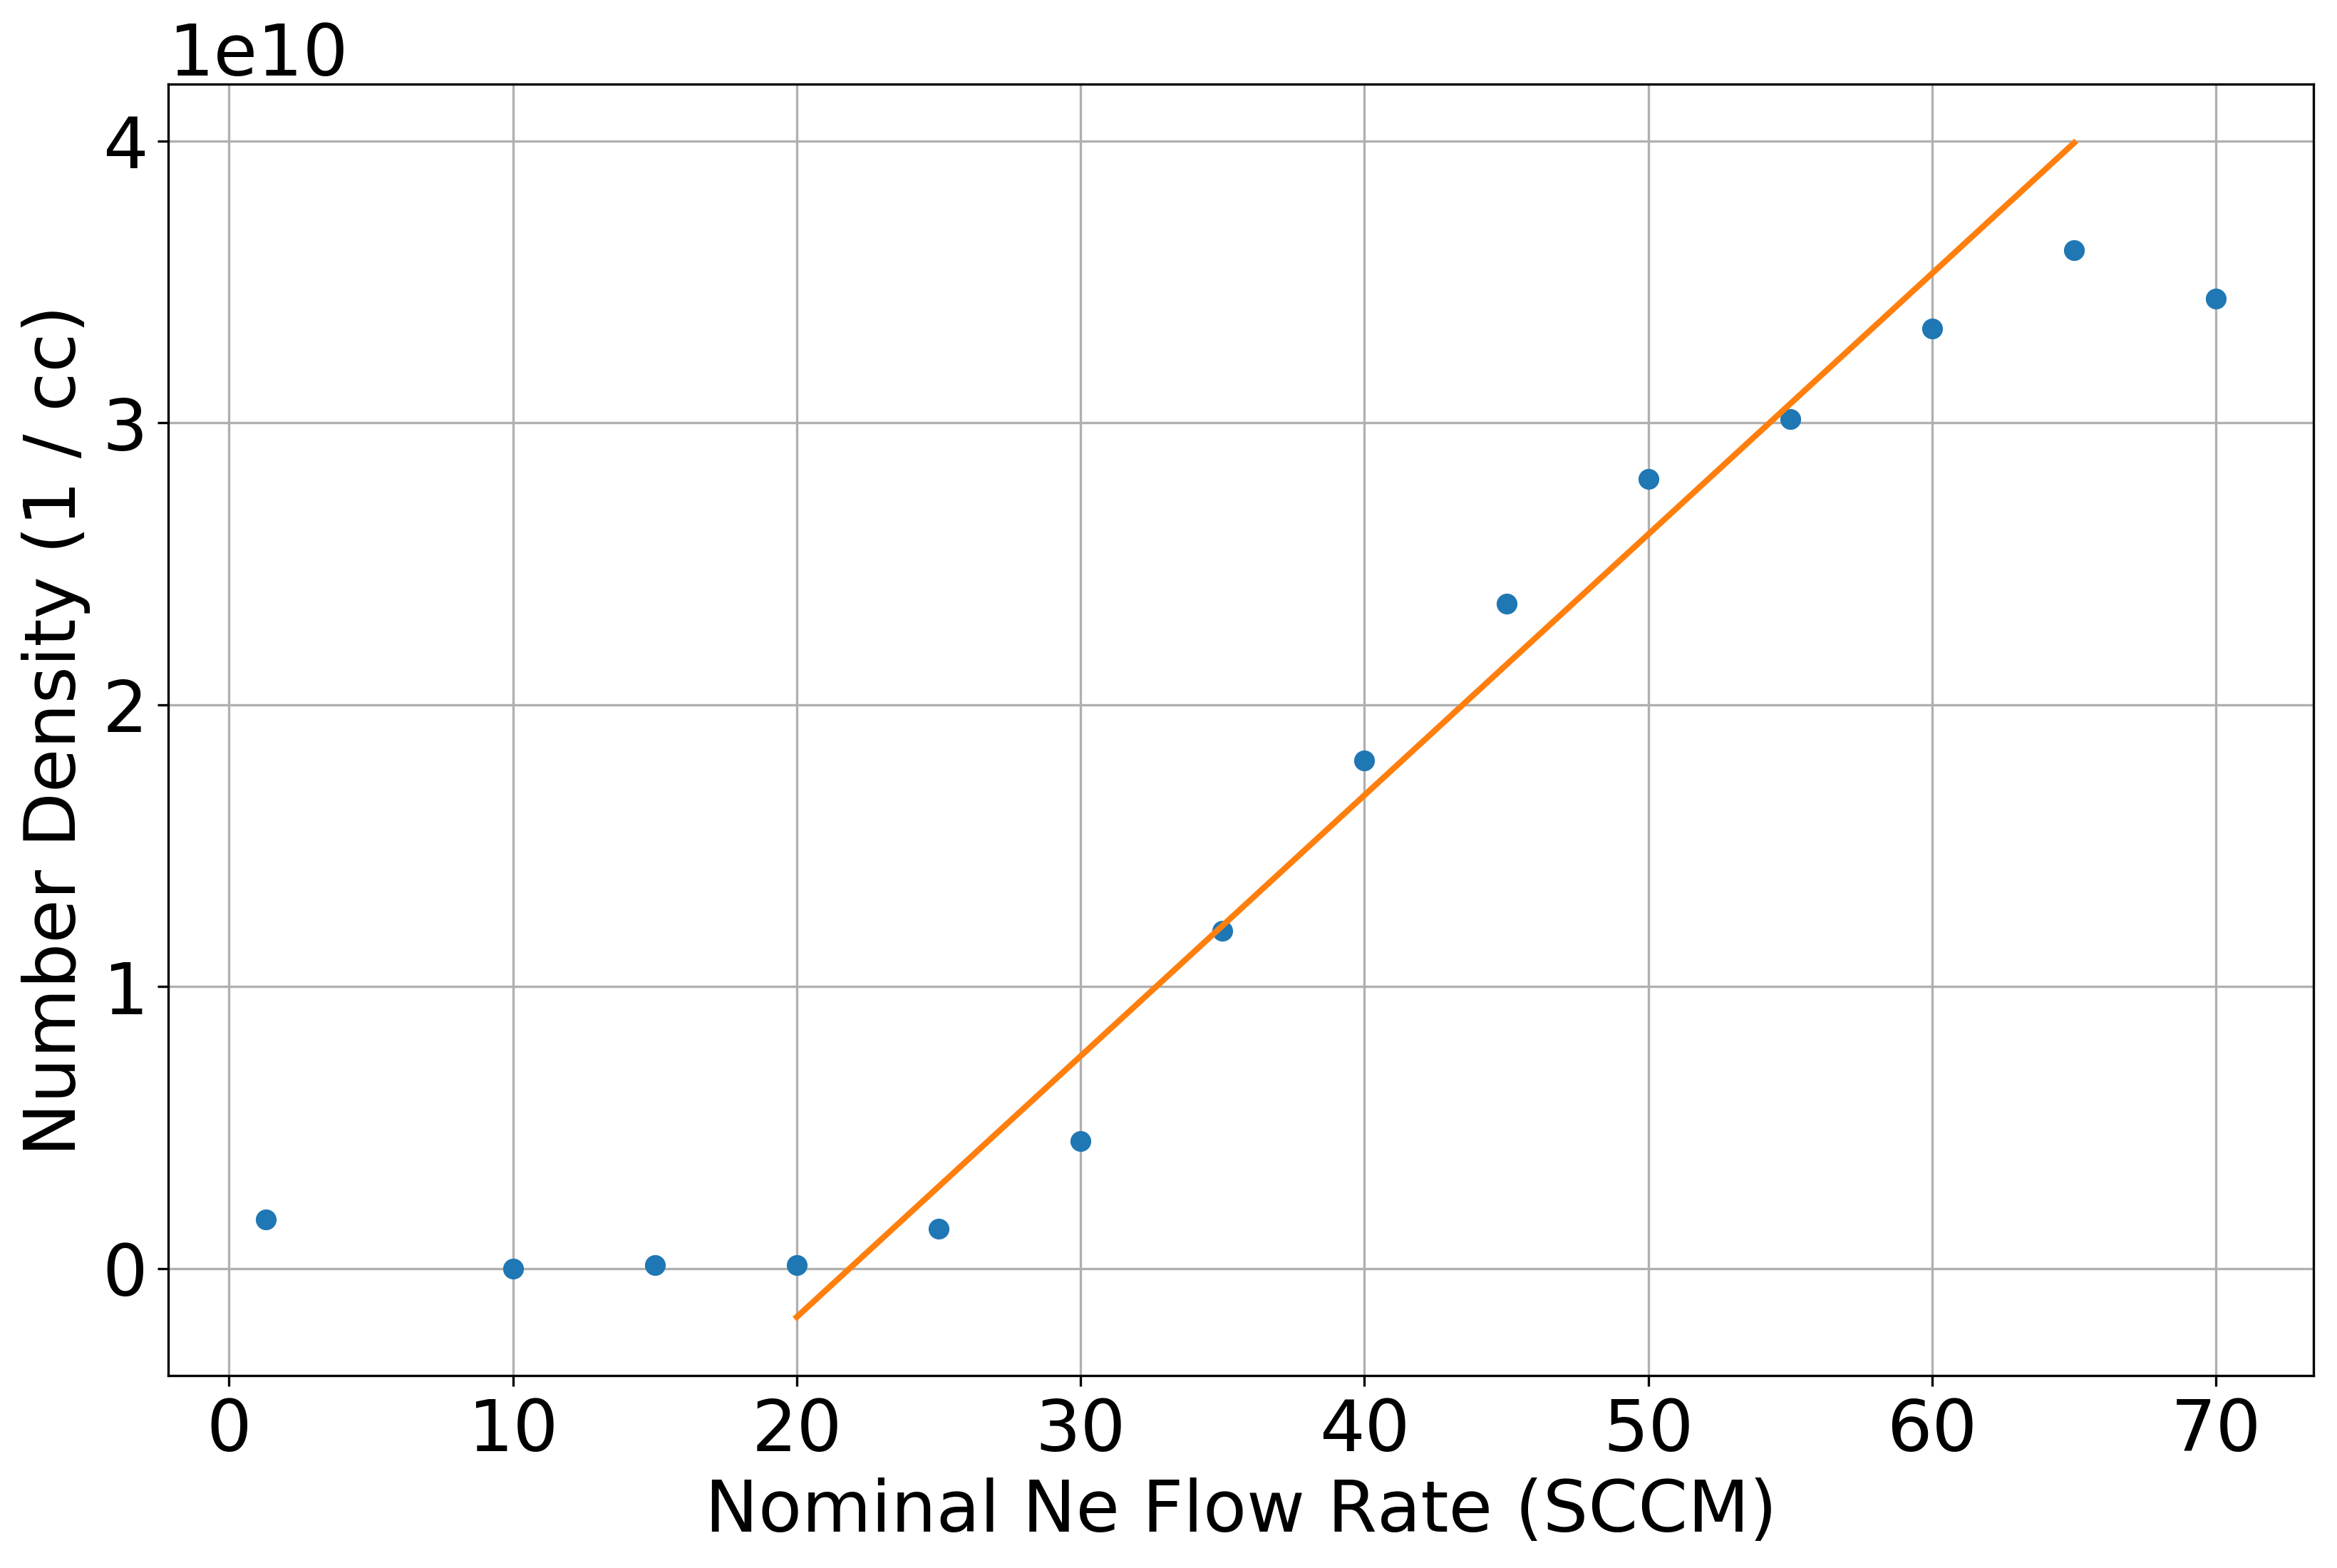
\includegraphics[width=1\textwidth]{images/CBGB_hydrodynamic_fit.png}
	\caption{$1.12 \times 10^9 x + -2.75 \times 10^10$}
	\label{f: rga}
\end{figure}

We know have previously calculated the possible number densities of the buffer gas with varying aperture sizes and flow rates. But now we can utilize those equations with the data on the target species to plot out the range of densities that we may see at the trap center as a function of the various apertures that we may utilize.

Knowing from our previous calculations:

\begin{align*}
	\bar{v} & = \sqrt{\frac{8 k_B T}{m \pi}} \\
	n_{0,b} & = \frac{4 f}{A_{aperture} \bar{v}} \\
	n(z) & = \frac{n_o}{2}\left(1-\frac{z}{\sqrt{z^2+a^2}}\right) \\
	\intertext{We can put it all together to get:} \\
	n(z) &= \alpha\frac{f}{A_{aperture} \bar{v}}\left(1-\frac{z}{\sqrt{z^2+a^2}}\right)
\end{align*}

But what we really care about is the region in which the number density is linearly dependent to the buffer gas flow rate, not over all possible ranges; we've seen that the target species only behaves linearly once it has been entrained in the buffer gas. This means that we should be equating the density function with the linear fit performed on the data for the parameters the data was taken at, $n(z)=mf+b$.

\begin{align*}
	\alpha & = \frac{m}{\beta}+\frac{b}{\beta f}
\end{align*}

Where we let $\beta = \frac{1}{A_{aperture, 0} \bar{v_0}}\left(1-\frac{z_0}{\sqrt{z_0^2+a_0^2}}\right)$. Thus, we may get a final form that incorporates the linear slope's dependence on the other variables of the system as well as the overall experimentally derived scaling factor from the data.

\begin{equation*}
	n(z) = \frac{mf+b}{A_{aperture} \bar{v} \beta}\left(1-\frac{z}{\sqrt{z^2+a^2}}\right)
\end{equation*}

There is a mass dependence in the thermal velocity equation, which leads us to conclude that the choice of the species is a statement of the effecacy of the beam itself. If we choose to calculate the thermal velocity of the target species found in the beam due to the theoretical thermal velocity of the buffer gas, that indicates that the beam properties are still dominated by the buffer gas species. This may not be the case, as we see in our data, we have a ratio of about 10:1, this is pushing the boundaries of the assumption that the buffer gas far outnumbers the target species. At these ratios, we may start to see the effects of the target species on the beam properties.

\begin{figure}[H]
	\centering
	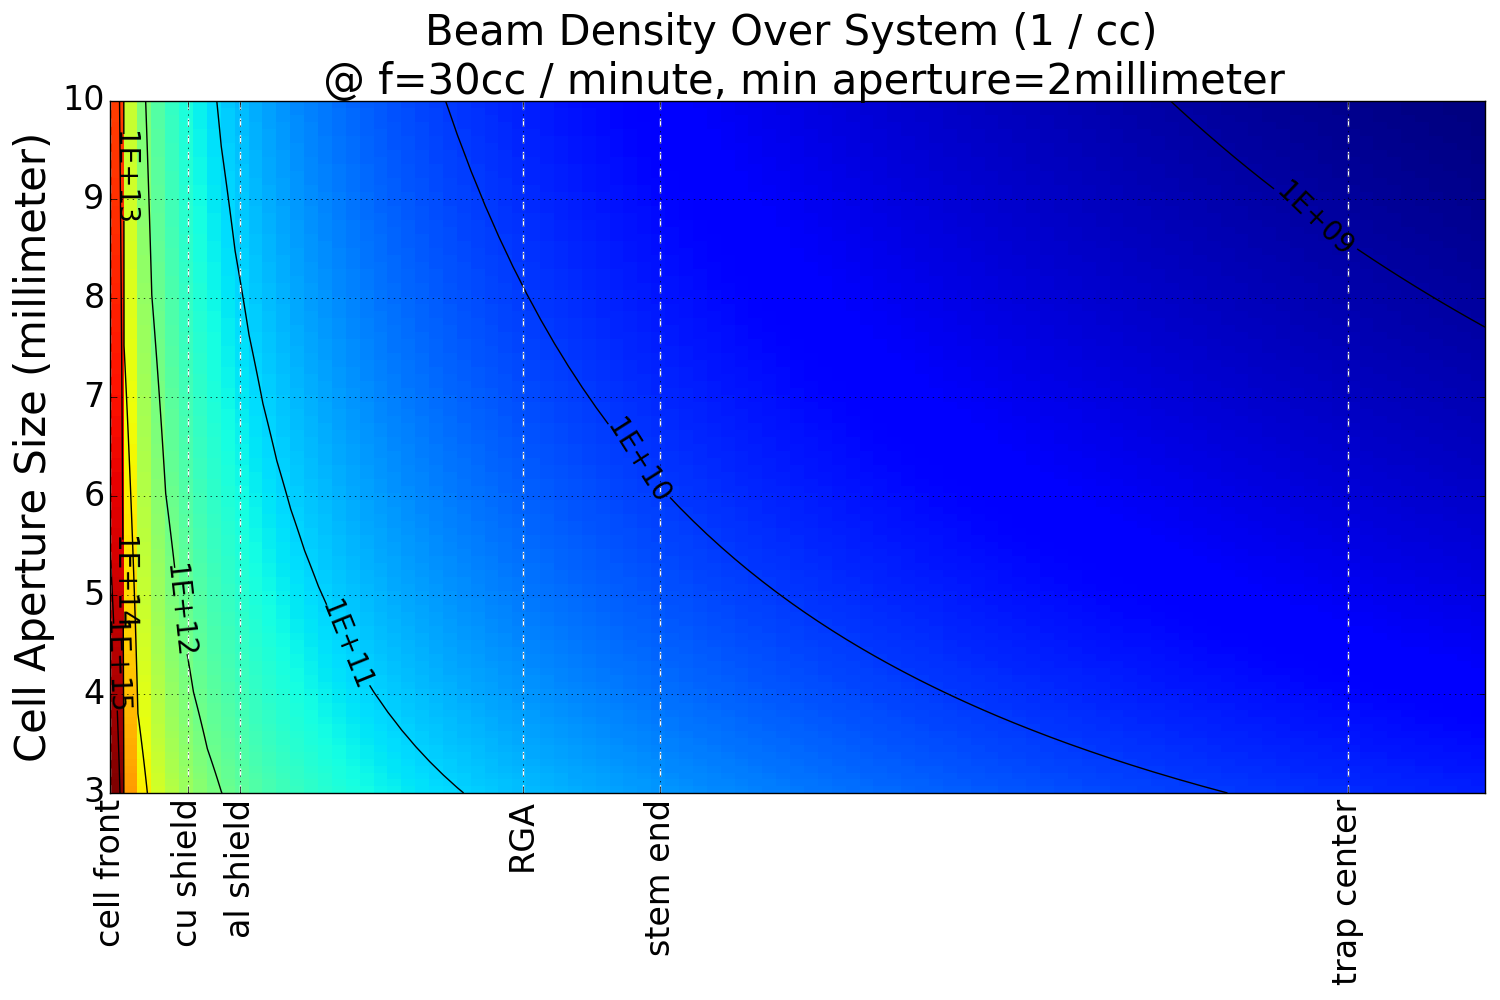
\includegraphics[width=1\textwidth]{images/CBGB_beam_density_over_system.png}
	\caption{Projected buffer gas beam densities with a Ne flow rate of 30SCCM with various distances of interest within the chamber. Optimal densities of entrained gasses hover around $0.1\%$ of the buffer gas value shown here.}
	\label{f: beam_density}
\end{figure}

Extrapolating the fit and estimated density from figure \ref{f: rga}, we can estimate the density of the water at various locations along the beam line as shown in figure \ref{f: beam_density}. We find that we should be able to produce an appreciable number density of water down at the trap center.

From the RGA, we were able to open and close a shutter in the beam path and see an extinction of the water signal, but a more accurate representation would be from the ions in the trap themselves. We know that the trapped $Be^+$ ions will reaction with $H_2O$ to predominately produce $BeOH$, which we see as a drop in the fluorescence. Figure \ref{f: shutter_closing} shows fits of the fluorescence decay as a beam from the CBGB is suddenly blocked by our shutter in the beam line. Comparing the fitted reaction rates, we find that they agree with the background rates found as shown in figure \ref{f: shutter_bkg}. This indicates to us that we indeed have a beam of cryogenic water coming from the CBGB, as seen by the sudden extinction of the $Be^+ + H_2O$ reaction.

\begin{figure}[H] \label{f: shutter_bkg}
	\centering
	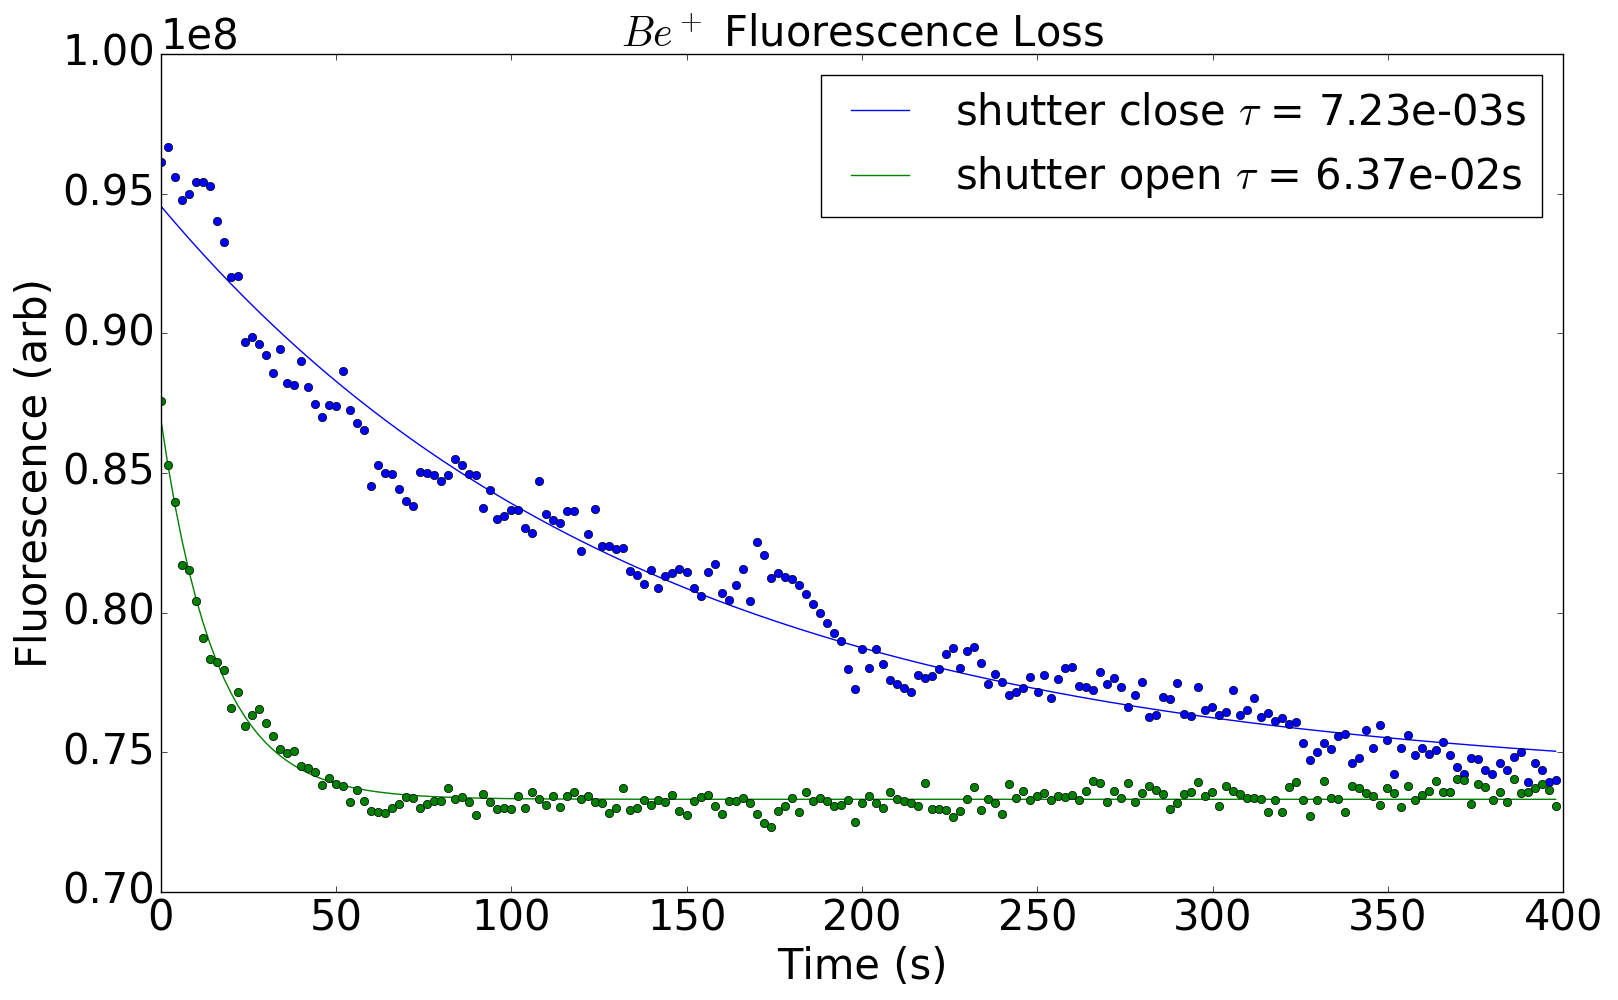
\includegraphics[width=1\textwidth]{images/CBGB_sudden_shutter_flow_bkg.png}
	\caption{}
\end{figure}

\begin{figure}[H] \label{f: shutter_closing}
	\centering
	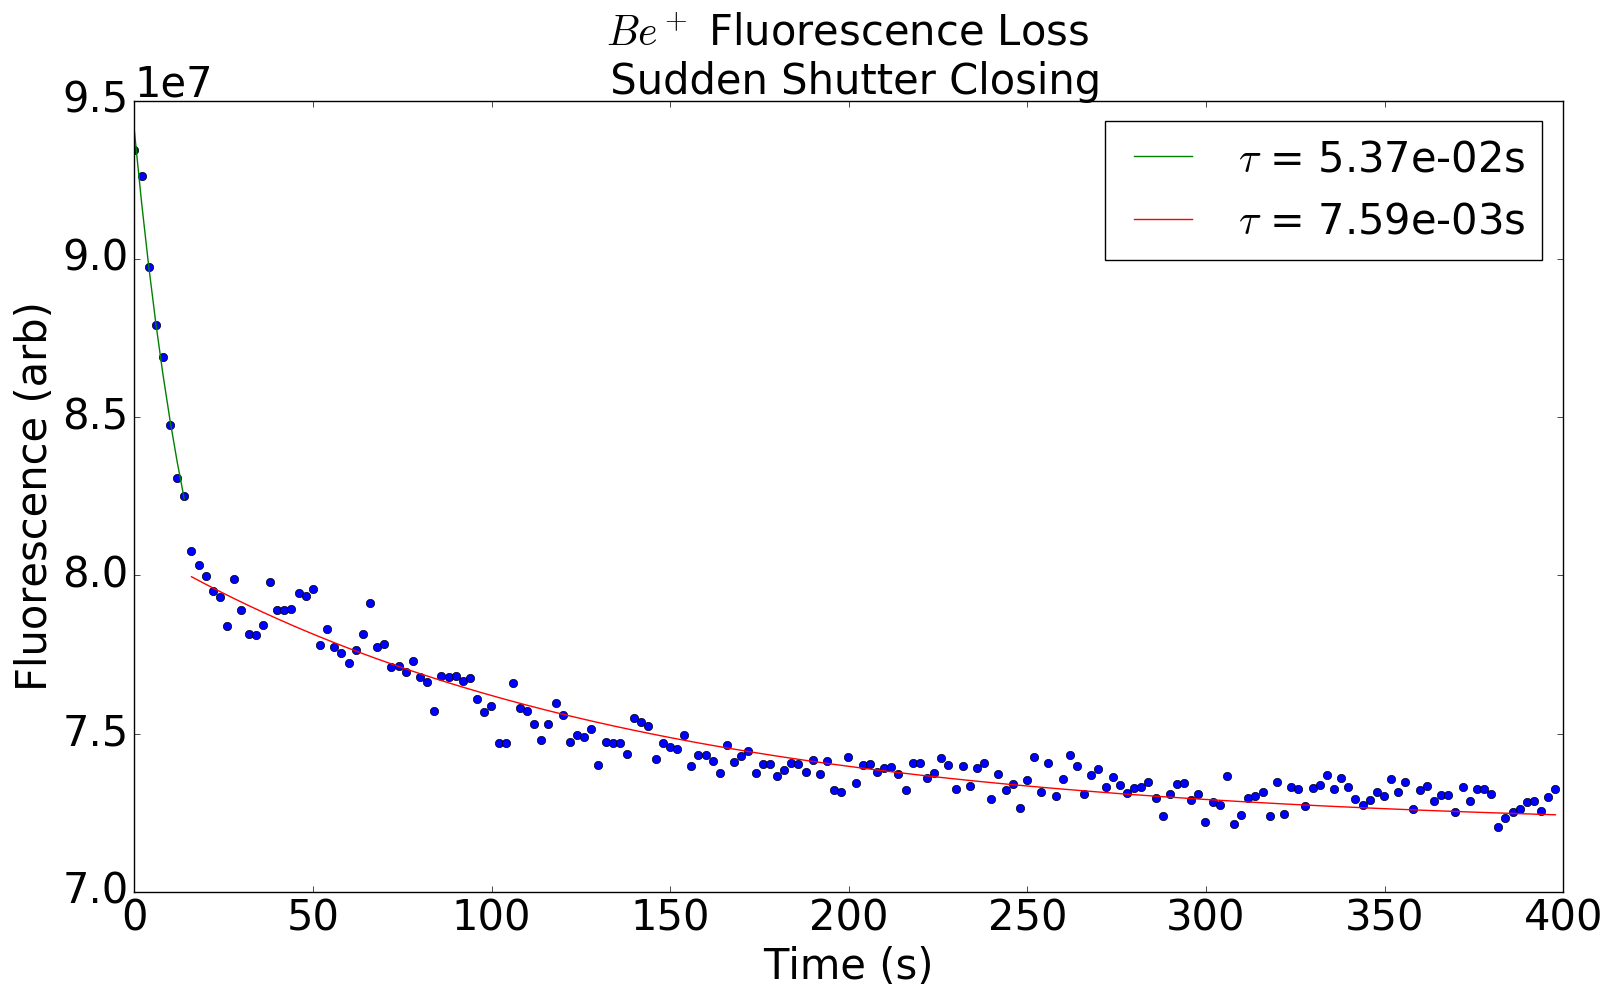
\includegraphics[width=1\textwidth]{images/CBGB_sudden_shutter_flow.png}
	\caption{}
\end{figure}